% --- LaTeX Presentation Template - S. Venkatraman ---

% --- Set document class ---

% Remove "handout" when presenting to include pauses
\documentclass[dvipsnames, handout]{beamer}
\usepackage{layout}
\usepackage{caption}
\usepackage{subcaption}
\usetheme{default}
\usepackage{textcomp}
\usepackage{pifont}
\usepackage{subcaption}
\usepackage{tabularx}
\usepackage[inline]{asymptote}


% Make content that is hidden by pauses "transparent"
\setbeamercovered{transparent}

% --- Slide layout settings ---

% Set line spacing
\renewcommand{\baselinestretch}{1.15}

% Set left and right text margins
\setbeamersize{text margin left=8mm, text margin right=8mm}


% Add slide numbers in bottom right corner
\setbeamertemplate{footline}[frame number]

% Remove navigation symbols
\setbeamertemplate{navigation symbols}{}

% Allow local line spacing changes
\usepackage{setspace}

% --- Color and font settings ---
% We will mainly use 2 colors: uofsc-red-primary, black
% We will use several font sizes to differentiate title, subtitle, normal text, etc.

\usepackage{xcolor}

% define theme colors
\definecolor{uofsc-red-primary}{HTML}{73000a}
\definecolor{uofsc-red-rose}{HTML}{cc2e40}
\definecolor{uofsc-red-dark}{HTML}{570008}

% Change itemized list bullets to circles
\setbeamertemplate{itemize item}{\color{uofsc-red-rose}$\bullet$}
\setbeamertemplate{itemize subitem}{\color{uofsc-red-rose}$\circ$}

\setbeamertemplate{enumerate item}{\color{uofsc-red-rose}\arabic{enumi}.}

% Slide title background color
\definecolor{background}{HTML}{ffffff}

% Slide title text color
\definecolor{titleText}{HTML}{73000a}

% Other possible color schemes

% - Light green/dark green -
%\definecolor{background}{HTML}{e4ede4}
%\definecolor{titleText}{HTML}{2e592f}

% - Light blue/dark blue -
%\definecolor{background}{HTML}{d5d9e8}
%\definecolor{titleText}{HTML}{2d375e}

% - Beige/dark blue -
%\definecolor{background}{HTML}{e8e2d5}
%\definecolor{titleText}{HTML}{2d3375}

% Set colors
\setbeamercolor{frametitle}{bg=background, fg=titleText}
\setbeamercolor{title}{fg=uofsc-red-primary}
\setbeamercolor{subtitle}{fg=uofsc-red-primary}

% Set font sizes for frame title and subtitle
\setbeamerfont{frametitle}{size=\fontsize{15}{16}}
\setbeamerfont{framesubtitle}{size=\small}

% --- Math/Statistics commands ---

% Add a reference number to a single line of a multi-line equation
% Usage: "\numberthis\label{labelNameHere}" in an align or gather environment
\newcommand\numberthis{\addtocounter{equation}{1}\tag{\theequation}}

% Shortcut for bold text in math mode, e.g. $\b{X}$
\let\b\mathbf

% Shortcut for bold Greek letters, e.g. $\bg{\beta}$
\let\bg\boldsymbol

% Shortcut for calligraphic script, e.g. %\mc{M}$
\let\mc\mathcal

% \mathscr{(letter here)} is sometimes used to denote vector spaces
\usepackage[mathscr]{euscript}

% Convergence: right arrow with optional text on top
% E.g. $\converge[p]$ for converges in probability
\newcommand{\converge}[1][]{\xrightarrow{#1}}

% Weak convergence: harpoon symbol with optional text on top
% E.g. $\wconverge[n\to\infty]$
\newcommand{\wconverge}[1][]{\stackrel{#1}{\rightharpoonup}}

% Equality: equals sign with optional text on top
% E.g. $X \equals[d] Y$ for equality in distribution
\newcommand{\equals}[1][]{\stackrel{\smash{#1}}{=}}

% Normal distribution: arguments are the mean and variance
% E.g. $\normal{\mu}{\sigma}$
\newcommand{\normal}[2]{\mathcal{N}\left(#1,#2\right)}

% Uniform distribution: arguments are the left and right endpoints
% E.g. $\unif{0}{1}$
\newcommand{\unif}[2]{\text{Uniform}(#1,#2)}

% Independent and identically distributed random variables
% E.g. $ X_1,...,X_n \iid \normal{0}{1}$
\newcommand{\iid}{\stackrel{\smash{\text{iid}}}{\sim}}

% Sequences (this shortcut is mostly to reduce finger strain for small hands)
% E.g. to write $\{A_n\}_{n\geq 1}$, do $\bk{A_n}{n\geq 1}$
\newcommand{\bk}[2]{\{#1\}_{#2}}

% Math mode symbols for common sets and spaces. Example usage: $\R$
\newcommand{\R}{\mathbb{R}}	% Real numbers
\newcommand{\C}{\mathbb{C}}	% Complex numbers
\newcommand{\Q}{\mathbb{Q}}	% Rational numbers
\newcommand{\Z}{\mathbb{Z}}	% Integers
\newcommand{\N}{\mathbb{N}}	% Natural numbers
\newcommand{\F}{\mathcal{F}}	% Calligraphic F for a sigma algebra
\newcommand{\El}{\mathcal{L}}	% Calligraphic L, e.g. for L^p spaces

% Math mode symbols for probability
\newcommand{\pr}{\mathbb{P}}	% Probability measure
\newcommand{\E}{\mathbb{E}}	% Expectation, e.g. $\E(X)$
\newcommand{\var}{\text{Var}}	% Variance, e.g. $\var(X)$
\newcommand{\cov}{\text{Cov}}	% Covariance, e.g. $\cov(X,Y)$
\newcommand{\corr}{\text{Corr}}	% Correlation, e.g. $\corr(X,Y)$
\newcommand{\B}{\mathcal{B}}	% Borel sigma-algebra

% Other miscellaneous symbols
\newcommand{\tth}{\text{th}}	% Non-italicized 'th', e.g. $n^\tth$
\newcommand{\Oh}{\mathcal{O}}	% Big-O notation, e.g. $\O(n)$
\newcommand{\1}{\mathds{1}}	% Indicator function, e.g. $\1_A$

% Additional commands for math mode
\DeclareMathOperator*{\argmax}{argmax}	% Argmax, e.g. $\argmax_{x\in[0,1]} f(x)$
\DeclareMathOperator*{\argmin}{argmin}	% Argmin, e.g. $\argmin_{x\in[0,1]} f(x)$
\DeclareMathOperator*{\spann}{Span}	% Span, e.g. $\spann\{X_1,...,X_n\}$
\DeclareMathOperator*{\bias}{Bias}	% Bias, e.g. $\bias(\hat\theta)$
\DeclareMathOperator*{\ran}{ran}		% Range of an operator, e.g. $\ran(T) 
\DeclareMathOperator*{\dv}{d\!}		% Non-italicized 'with respect to', e.g. $\int f(x) \dv x$
\DeclareMathOperator*{\diag}{diag}	% Diagonal of a matrix, e.g. $\diag(M)$
\DeclareMathOperator*{\trace}{trace}	% Trace of a matrix, e.g. $\trace(M)$
\DeclareMathOperator*{\supp}{supp}	% Support of a function, e.g., $\supp(f)$

% --- Presentation begins here ---

\begin{document}

% --- Title slide ---
% We have to specify the location of title, subtitle, author, dates, institutes, etc
% Right now we just put everything on the slides, without specifying the space between rows or the height of blocks.
% We will fix these details later.
% In general, we don't want to have too many different font sizes to mess up a page. The names, dates, affiliations (institutes, emails) should be of the same font size, except for some extreme cases (for example, the affiliation is too long and it has to be shrank to be fitted into the page).
% The space between title (including subtitle) to author to affiliation should keep constant. It's not the absolute location but the space in between that determines the overall look of the page.
% We will design this better, with reference to https://www.overleaf.com/learn/latex/Beamer


\title{mmMIC: Multi-modal Speech Recognition based on mmWave Radar}

\author{Fan et al., 2023 INFOCOM \\(to appear)\vspace{-.3cm}}

%\institute{University of South Carolina}
\date{05/10/2023}

\begin{frame}
\titlepage
\vspace{-1.2cm}
\begin{center}
%
\includegraphics[width=1cm]{imgs/uofsc-logo.png}\bigskip
%{\begin{spacing}{1.2}\scriptsize 
%Joint work with FirstName LastName, FirstName LastName
%\end{spacing}}
\end{center}
\end{frame}

% --- Main content ---

% Example slide: use \pause to sequentially unveil content
\begin{frame}[t]{Motivation}
%\framesubtitle{Collecting data from consumer wearables}

\begin{itemize}
\item Speech recognition has a wide range of applications
\begin{enumerate}
\item Smart driving 
\item Smart home
\item Smart medical care
\item other
\end{enumerate}

\item Limitations of Existing Solutions
\begin{enumerate}
\item Microphone-based solutions suffer from multi-source interference 
\item Single-sensor approaches fail to achieve great performance
\item Multi-sensor approaches incur additional device cost
\end{enumerate}


\item mmMic
\begin{enumerate}
\item Low cost, great performance, privacy preserved
\end{enumerate}
\end{itemize}
\end{frame}

\begin{frame}[t]{Main Ideas of mmMIC}
%\framesubtitle{Collecting data from consumer wearables}

\begin{enumerate}
\item Extract macro-motion features from lip motions (Doppler Velocity)
\item Extract micro-vibration features from vocal-cords vibrations (Spectrogram)
\item Fusion both features for speech recognition (TransFuser)
\end{enumerate}

\begin{center}
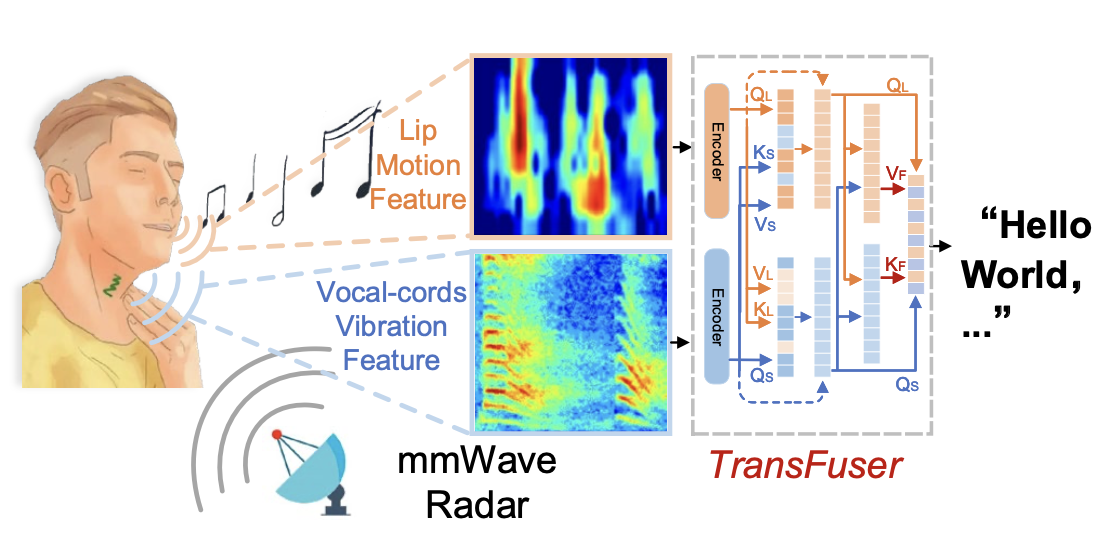
\includegraphics[width=0.75\textwidth]{imgs/mmmic-fig1.png}
\end{center}

\end{frame}

\begin{frame}[t]{Empirical Study: Sensing Lip Motion with FMCW Radar}
%\framesubtitle{Empirical study}

\begin{itemize}
\item Apply Range-FFT and Doppler-FFT on the IF signals
\item The lip motion info is perceived with the phase velocity feature
\item The angular frequency $w$ of phase changing:
$$w = 2\pi f_d = \frac{4\pi v_r}{\lambda}, $$
where $f_d$ is the Doppler shift, $v_r$ is the target velocity.
\end{itemize}

\begin{center}
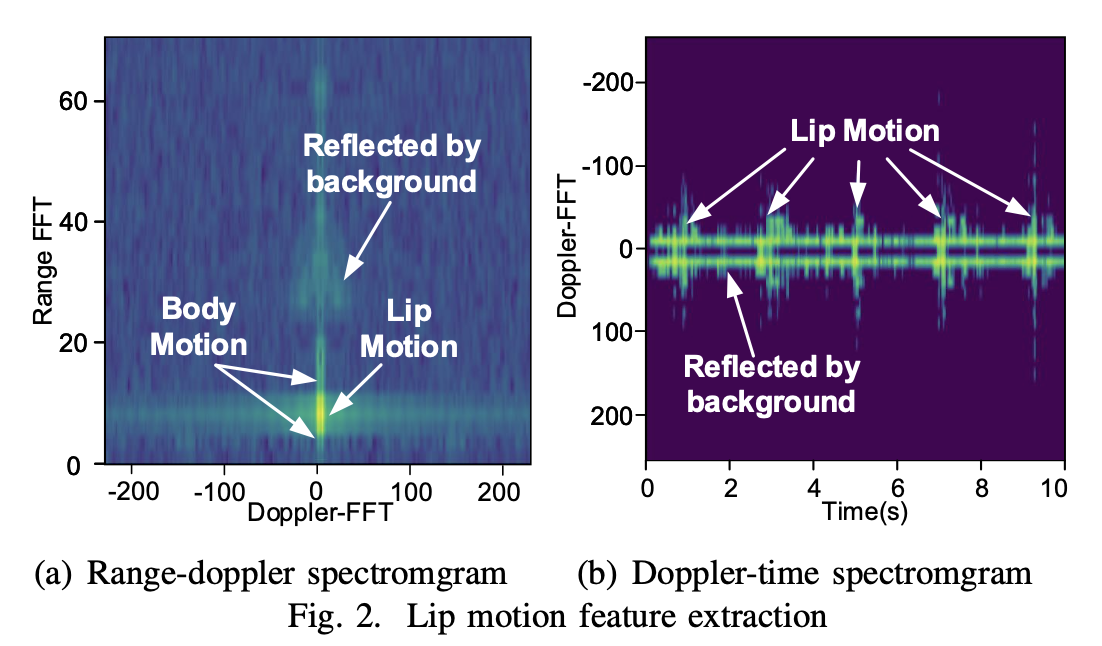
\includegraphics[width=0.65\textwidth]{imgs/mmmic-fig2.png}
\end{center}

\end{frame}

\begin{frame}[t]{Sensing Lip Motion -- Examples}
\begin{itemize}
\item Lip motions of 8 different phonetic symbols are perceived by mmWave radar
\end{itemize}
\begin{center}
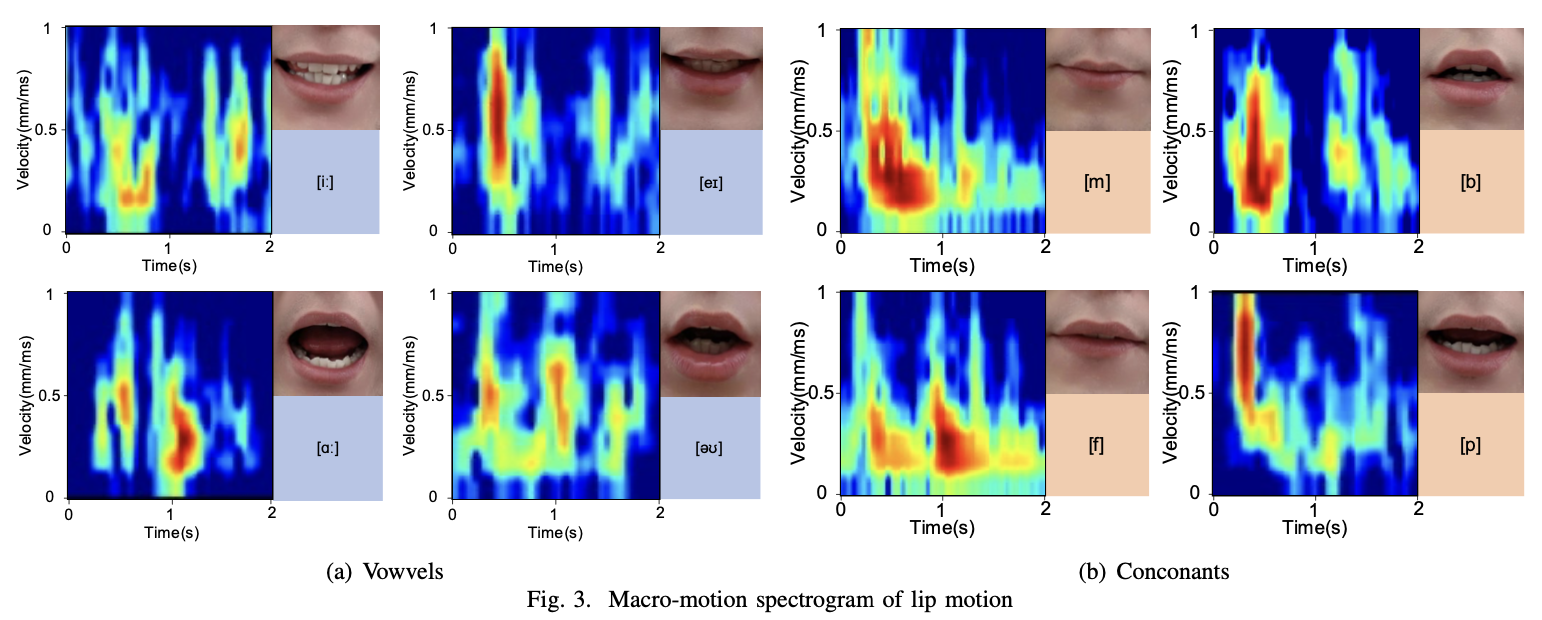
\includegraphics[width=0.9\textwidth]{imgs/mmmic-fig3.png}
\end{center}
\end{frame}


\begin{frame}[t]{Empirical Study: Sensing Vocal-cords with FMCW Radar}
%\framesubtitle{Collecting data from consumer wearables}

\begin{itemize}
\item Collect speech signal with both mmWave radar and microphone
\item Apply Range-FFT and Doppler-FFT on the IF signals
\item Use a high-pass filter to remove lip/head motion interference
\end{itemize}

\begin{center}
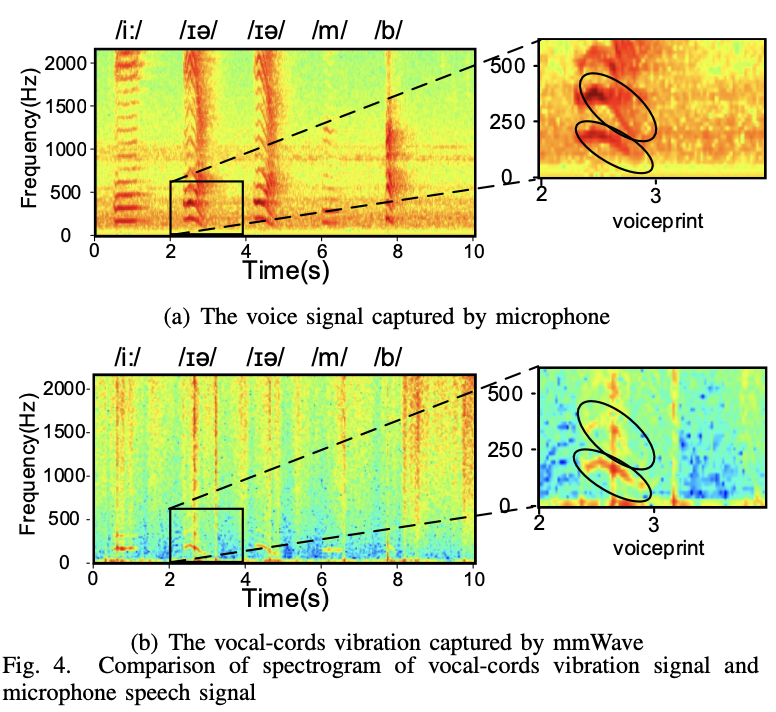
\includegraphics[width=0.6\textwidth]{imgs/mmmic-fig4.png}
\end{center}

\end{frame}


\begin{frame}[t]{Empirical Study: Conclusions}
%\framesubtitle{Collecting data from consumer wearables}

\begin{enumerate}
\item Lip motion characteristics:
\begin{itemize}
\item Low frequency, large amplitude, high velocity
\item Extract features by doppler-velocity spectrogram
\end{itemize}
\item Vocal-cords characteristics: 
\begin{itemize}
\item High frequency, small vibration amplitude
\item Extract features by frequency-time spectrogram
\end{itemize}
\end{enumerate}

\end{frame}


\begin{frame}[t]{System Design: Overview}
%\framesubtitle{A mmWave-based multi-modal fusion lip-vibration speech recognition system}

\begin{itemize}
\item Extracting macro-motion features:
\begin{itemize}
\item Doppler-velocity spectrogram + difference-based interference removal
\end{itemize}

\item Extracting micro-vibration features:
\begin{itemize}
\item Phase change from frequency-time spectrogram + cross verification with lip motion
\end{itemize}

\item Attention-based multi-modal fusion and recognition
\end{itemize}

\begin{center}
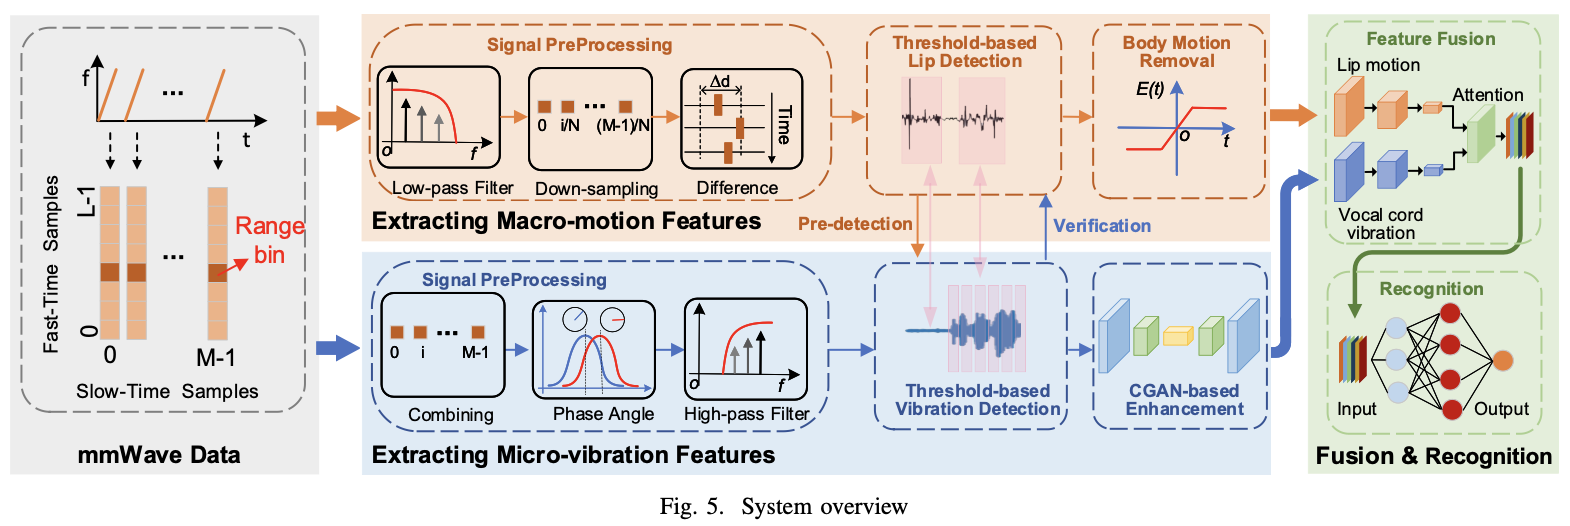
\includegraphics[width=0.95\textwidth]{imgs/mmmic-fig5.png}
\end{center}

\end{frame}

\begin{frame}[t]{System Design: Extracting Macro-motion Features}
%\framesubtitle{Collecting data from consumer wearables}

\begin{enumerate}
\item Signal preprocessing/modeling: 
$$S = S_v + S_l + S_d + S_b, \qquad S_{l+d} = S_l + S_d,$$
$S$: all reflected signals at the receiver; $S_b$: background static interference signals (cancelable); $S_d$: dynamic interference from head/body motion;   $S_l$: lip motion signals; $S_v$: vocal-cords vibration signals (low-pass filtered + down-sampling). 
\end{enumerate}

\begin{center}
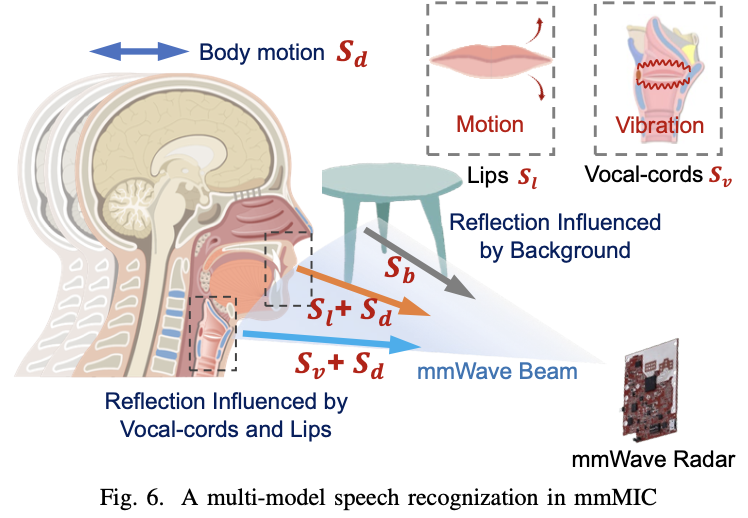
\includegraphics[width=0.45\textwidth]{imgs/mmmic-fig6.png}
\end{center}

\end{frame}

\begin{frame}[t]{System Design: Extracting Macro-motion Features}
%\framesubtitle{Collecting data from consumer wearables}

\begin{enumerate}
\setcounter{enumi}{1}
\item Dynamic Interference Removal
\begin{itemize}
\item Dynamic interference estimation:
$$\hat{S}_d = \frac{1}{2N}\sum^N_{n=-N} \alpha_n \cdot S_{l+d}(R+n), \quad n, N\in \mathbb{Z}, n\ne 0,$$
where $\hat{S}_d$ is the estimated signal of dynamic interference; $S_{l+d}(R)$ is the lip motion signal including dynamic interference at range bin $R$; $2N$ is the total number of adjacent bins; $\alpha_n$ is the weight of the signal in the $n$-th bin and $\sum \alpha_i = 1$. 
\item STFT difference:
$$STFT(S_l) = STFT(S_{l+d}) - STFT(\hat{S}_d).$$
\end{itemize}
\end{enumerate}

\end{frame}



\begin{frame}[t]{System Design: Extracting Micro-vibration Features}
%\framesubtitle{Collecting data from consumer wearables}

\begin{enumerate}
\item Signal preprocessing: use high-pass filter to filter all low frequency signals.
\item Speech activity detection based on cross-validation.
\begin{itemize}
\item Split lip motion window into segments
\item Compute vocal-vibration signal energy for segments (sliding)
\item SVM to classify speech vs non-speech 
\end{itemize}
\item CGAN-based enhancement
\end{enumerate}

\begin{center}
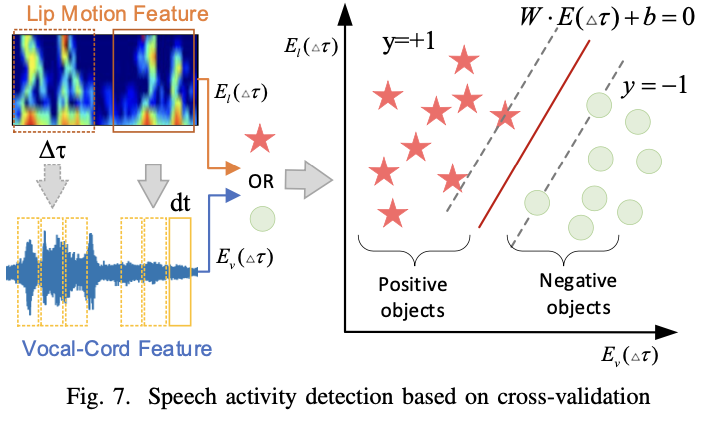
\includegraphics[width=0.65\textwidth]{imgs/mmmic-fig7.png}
\end{center}

\end{frame}

\begin{frame}[t]{System Design: Fusion \& Recognition (TransFuser)}
\framesubtitle{Leverage the self-attention mechanism of transformers}

\begin{enumerate}
\item Vocal-cords Vibration Encoder
\item Lip Motion Encoder
\item Multi-modal Fusion: complementarity between two modalities
\item Speech Recognition: decoder
\end{enumerate}


\begin{figure}[ht]
\begin{subfigure}[b]{0.4\textwidth}
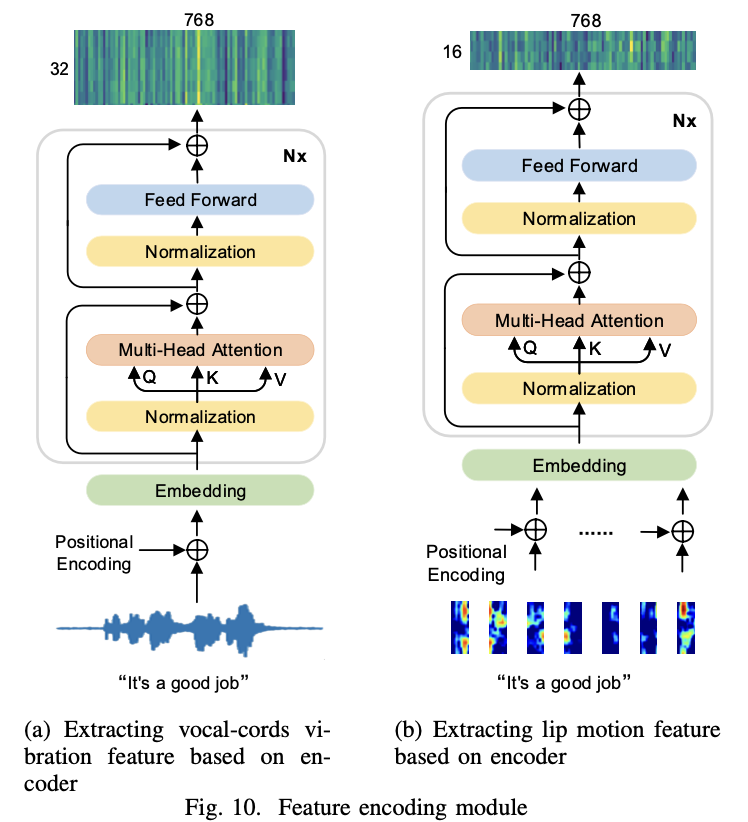
\includegraphics[width=\textwidth]{imgs/mmmic-fig10.png}
\end{subfigure}
\begin{subfigure}[b]{0.42\textwidth}
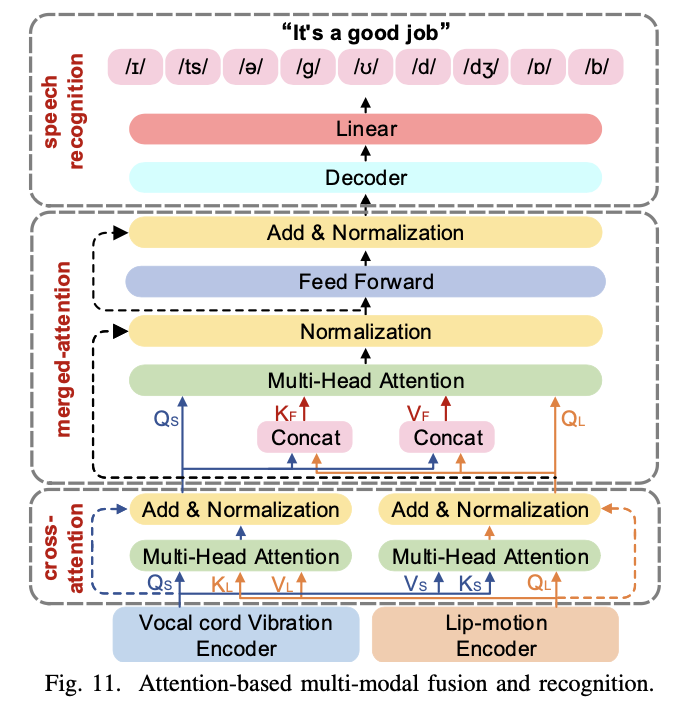
\includegraphics[width=\textwidth]{imgs/mmmic-fig11.png}
\end{subfigure}
\end{figure}

\end{frame}


\begin{frame}[t]{Evaluation Setup}
\begin{itemize}
\item Hardware: IWR6843BOOST: 60GHz; chirp duration: 50us; Sampling rate: 4000k; 64 samples per chirp.

\item Software: python script controlling both mmWave radar and microphone; lip encoder: 6 layers; hidden layer size 384; attention heads: 6; drop out rate: 0.2; adam optimizer $\beta=0.9, l_{rate}=1e-4$; weight decay: 100; batch size: 32.
\end{itemize}

\begin{center}
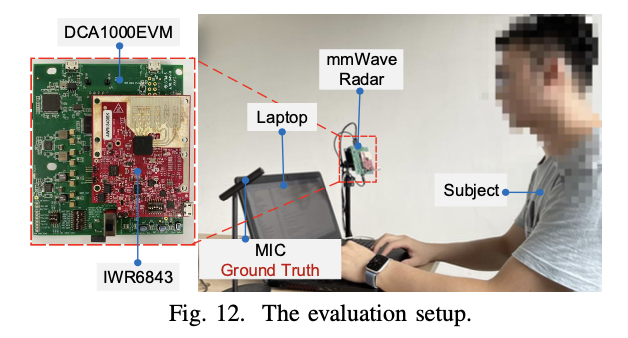
\includegraphics[width=0.65\textwidth]{imgs/mmmic-fig12.png}
\end{center}



%\begin{figure}[ht]
%\begin{subfigure}[b]{0.4\textwidth}
%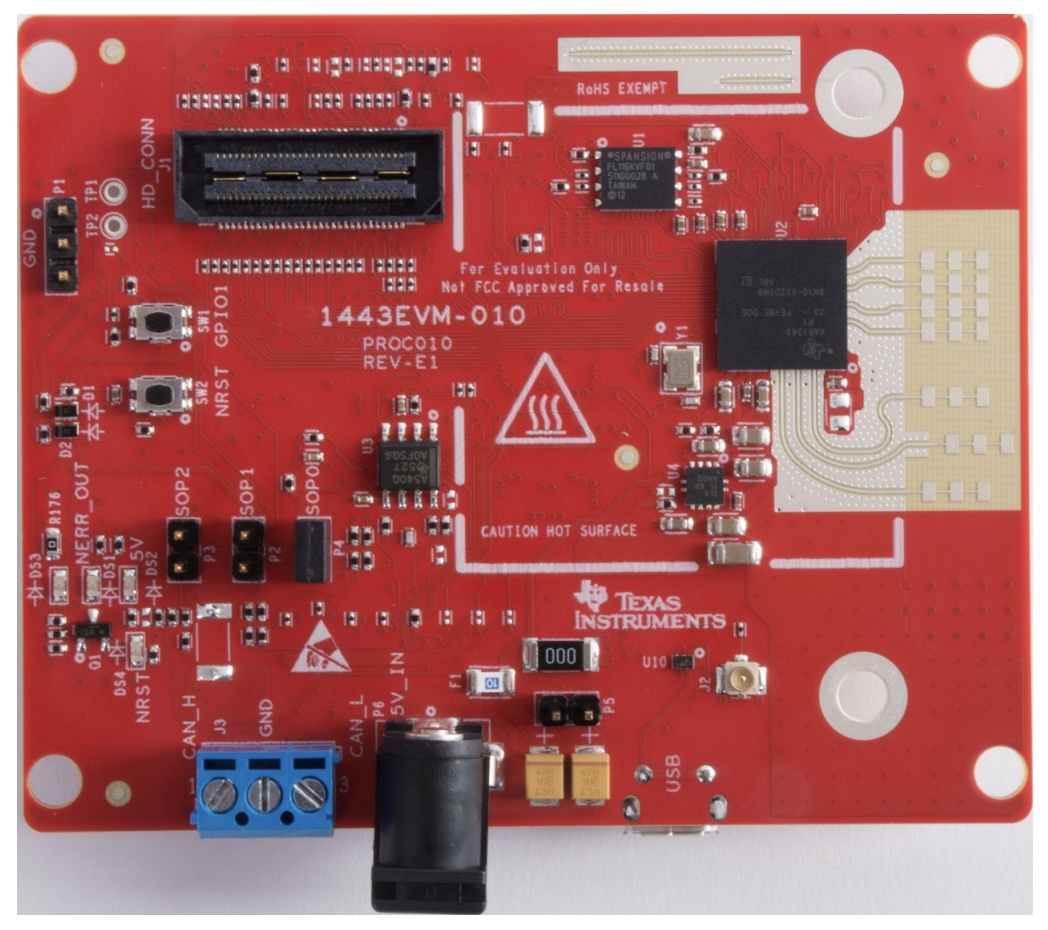
\includegraphics[width=\textwidth]{imgs/iwr1443boost.jpg}
%\end{subfigure}
%\begin{subfigure}[b]{0.4\textwidth}
%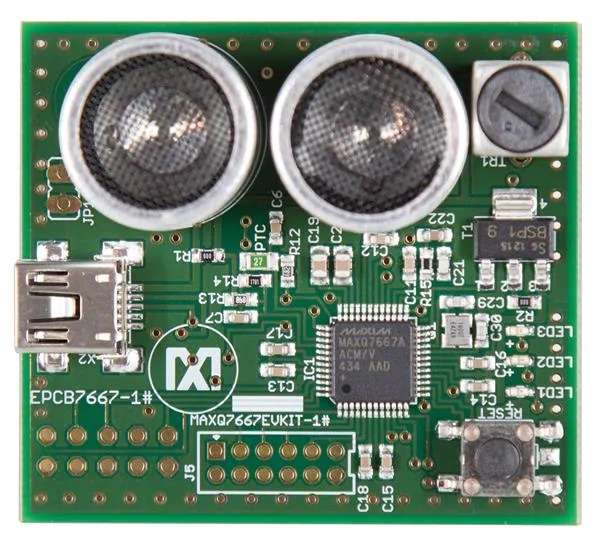
\includegraphics[width=\textwidth]{imgs/maxq7667evkit.jpg}
%\end{subfigure}
%\end{figure}

\end{frame}



\begin{frame}[t]{Evaluation Setup}
\begin{itemize}
\item Dataset: 
\begin{enumerate}
\item 48 phonetic symbols
\item 15 volunteers (8 male, 7 female)
\item 21600 sets of data (speech signals, vocal-cords vibration signals, lip motion signals)
\item Choose $\frac{1}{5}$ of the dataset to train, and predict the rest.
\end{enumerate}
\item Metrics
\begin{enumerate}
\item Accuracy: correctly identify samples in all samples
\item Recall: correctly identified samples out of total samples in each class
\end{enumerate}
\end{itemize}


\end{frame}


\begin{frame}[t]{Performance}
\begin{itemize}
\item Overall performance: over 96\% accuracy for all phonetic symbols (Fig 13a); above 85\% recall rate (Fig 13b).
\item Impact of Distance vs. Orientation: (Fig 13c, 13d, 13e) over 90\% accuracy.
\item Impact of Ambient Noises: (Fig 13f) over 90\% accuracy.
\item Impact of Multi-human: (Fig 13g) no major impact.
\item Impact of Body Motion: (Fig 13h) error increases proportionally. 
\end{itemize}

\begin{center}
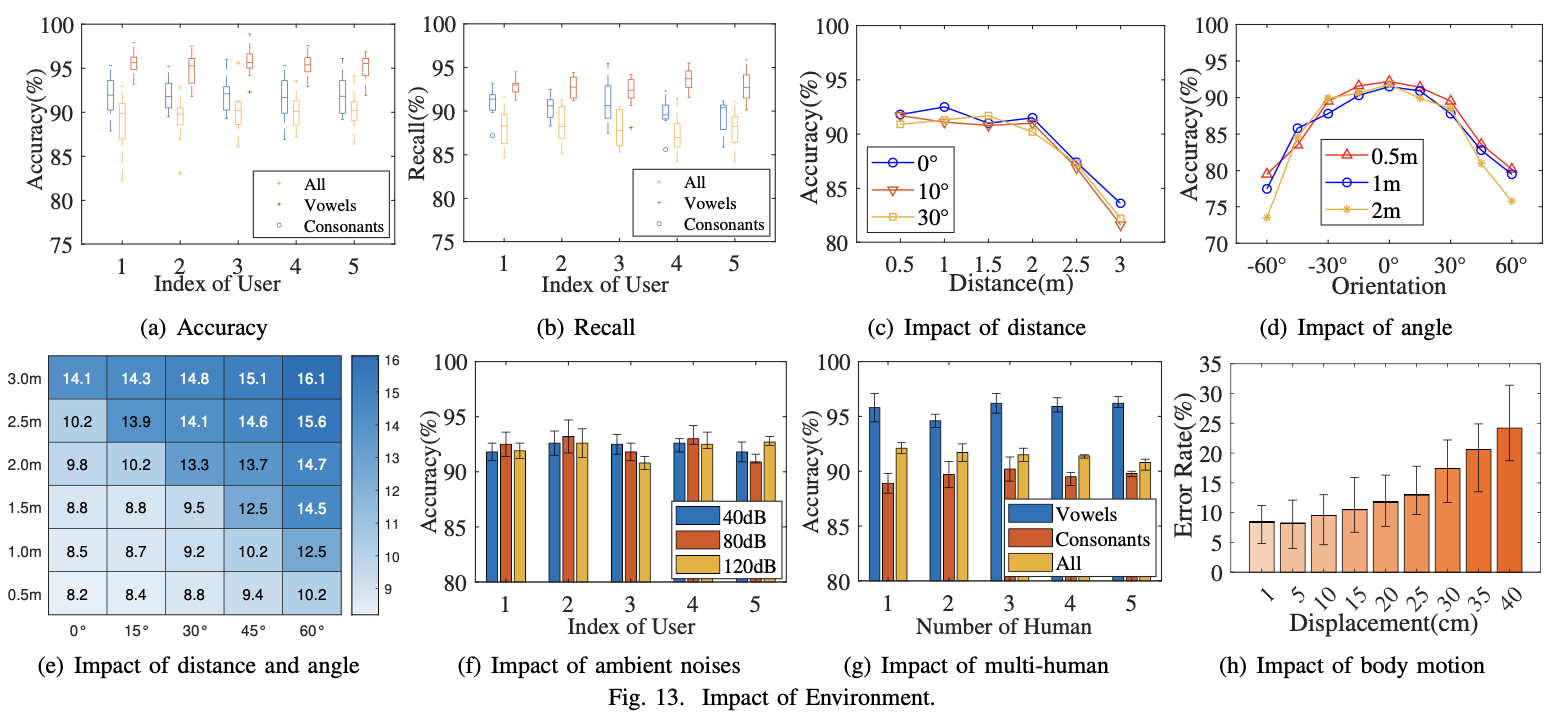
\includegraphics[width=0.85\textwidth]{imgs/mmmic-fig13.png}
\end{center}


\end{frame}


% --- Bibliography slide ---

%\begin{frame}{References}
%\begin{thebibliography}{10}
%\beamertemplatearticlebibitems
%{\small

%\bibitem{Paper1}
%Paper 1 Title.
%\newblock Paper 1 Authors. \\
%{\it Journal Name} Edition, Year.

%\bibitem{Paper 2}
%Paper 2 Title.
%\newblock Paper 2 Authors.\\
%arXiv:1234.56789.
%}
%\end{thebibliography}
%\end{frame}

% --- Thank you slide ---

%\begin{frame}
%\begin{center}
%{\large\color{titleText} Thank you!}
%\vspace{1cm}

%Zifei (David) Zhong \\[1em]
%zhongz@email.sc.edu \\
%https://zfz.github.io
%\end{center}
%\end{frame}

% --- Presentation ends here ---

\end{document}
